\section{Experiments}
\label{sec:exp}

\subsection{Dataset}
\label{sec:data}

FIRC2234 is a single-rail referring-segmentation corridor set of ego-view rail frames, all $550{\times}550$ pixels, split by original image ID into 1664/208/208 train/val/test frames with no overlap.
Every frame contains exactly one rail polygon and carries an ordinal caption; the val and test splits use a single caption string each (``near first from left rail track in frame''), and the train split contains two distinct strings across 1664 frames.
The referred rail occupies a median $4.7\%$ of the image (p10--p90 $3.2$--$7.3\%$ on test), i.e.\ a thin perspective corridor rather than a compact object, precisely the regime in which a dense, arbitrary-shaped mask decoder is a poor carrier.
Table~\ref{tab:data} summarizes the protocol, and Figure~\ref{fig:dataset} shows both the resulting distributions and six sample frames.
Training uses the 1664 original frames \emph{and} their horizontal flips (3328 frames): images, masks, and $\phih^{gt}$ are mirrored and the caption's spatial words are swapped accordingly, while photometric jitter is online and does not write extra files.
Val and test remain the original 208+208 images and captions, all numbers below that are not marked as transfer are computed on this 208-frame test split, and all evaluation is fp32.

\begin{figure*}[t]
\centering
\IfFileExists{figures/fig2_firc_dataset.pdf}{%
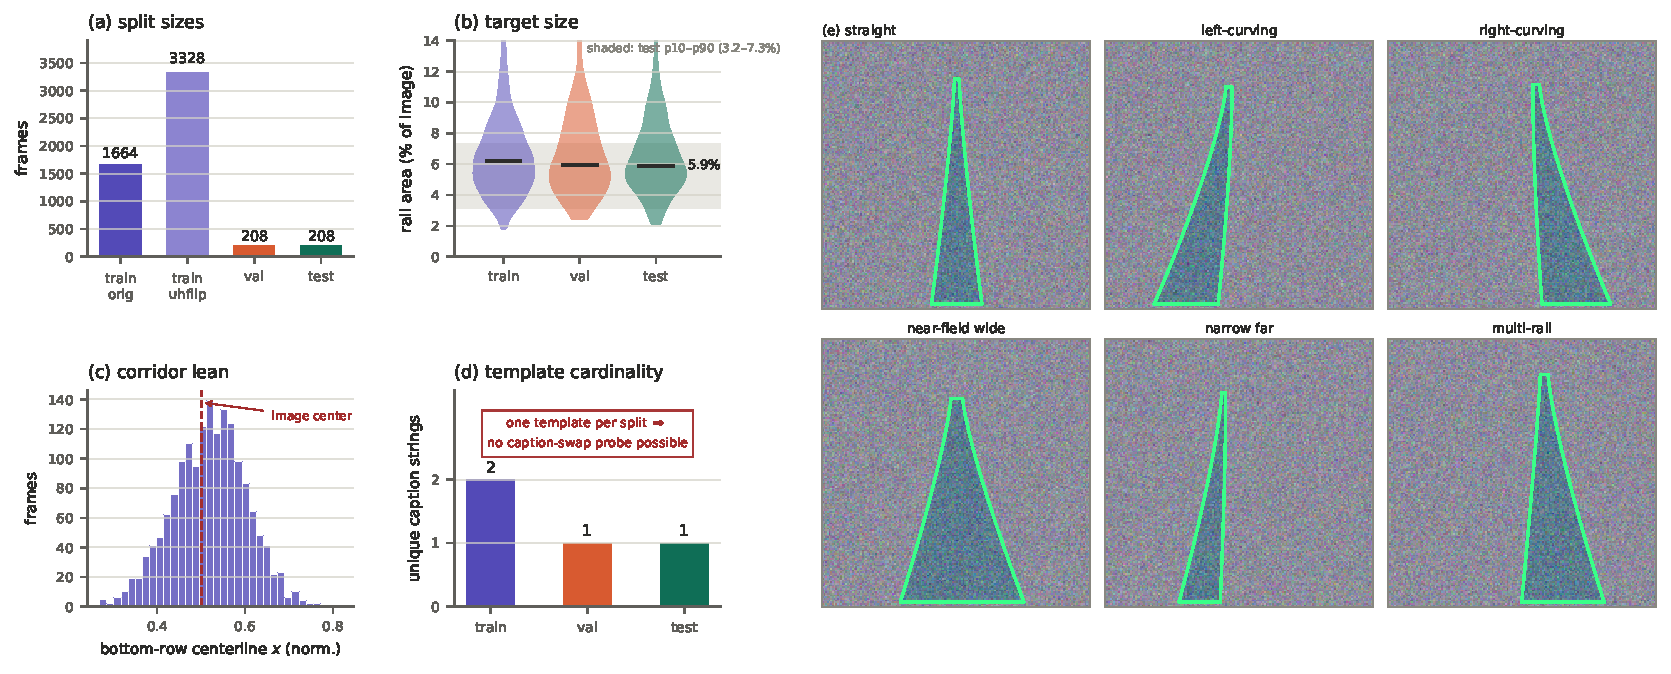
\includegraphics[width=\textwidth]{figures/fig2_firc_dataset.pdf}%
}{%
\fbox{\parbox{0.95\textwidth}{\centering\vspace{14mm}Dataset panel omitted in this build.\vspace{14mm}}}%
}%
\caption{FIRC2234 at a glance.
(a)~split sizes, including the $\times2$ horizontal-flip doubling that the train split receives.
(b)~the rail-area distribution per split, the mask-to-image ratio whose p10--p90 range on test ($3.2$--$7.3\%$) is the thin-corridor regime the carrier is designed for.
(c)~the horizontal position of the corridor centerline on the bottom image row, a proxy for how far the corridor leans out of the image axis: the spread is what a $20$-D carrier must cover.
(d)~the number of distinct caption strings per split; a single eval template is why no caption-swap linguistic probe can be run on this dataset (Section~\ref{sec:transfer}).
(e)~six test-style frames spanning the split, with the ground-truth rail polygon in green; from left to right, top to bottom: straight, left-curving, right-curving, the widest near-field frame, a narrow far-field corridor, and a multi-rail ordinal frame.
Panels (a)--(d) are computed from the released annotations; panel (e) is rendered from the annotation geometry.}
\label{fig:dataset}
\end{figure*}

\begin{table}[t]
\centering
\small
\setlength{\tabcolsep}{4pt}
\caption{FIRC2234 protocol. All frames are $550{\times}550$; statistics are computed from the released annotations. Rail area is the mask-to-image ratio (test p10--p90 $3.2$--$7.3\%$). Val and test each use one caption string; the train split uses two.}
\label{tab:data}
\begin{tabularx}{\columnwidth}{@{}lYcc@{}}
\toprule
Split & Role & Frames & Rail area (med.) \\
\midrule
train & orig $\cup$ hflip & 1664 ($\times2$) & $4.7\%$ \\
val & eval & 208 & $4.7\%$ \\
test & eval & 208 & $4.7\%$ \\
\bottomrule
\end{tabularx}
\end{table}

\subsection{Setup}
\label{sec:setup}

\textbf{The reference set.}
FIRC2234 is introduced in this work; consequently, to our knowledge, \emph{no previously published method has been trained on it}.
The comparison set therefore consists of the strongest \emph{off-the-shelf} systems that apply to ego-view rail frames without task-specific adaptation---the same set a practitioner faces at deployment time.
We report gIoU (mean per-frame mask IoU), \PrAt{0.5} and \PrAt{0.7} (the share of frames with IoU ${\ge}0.5$ and ${\ge}0.7$), and SegRate (fraction of frames with any predicted mask).
The reference rows are all off-the-shelf, measured by us on the same protocol: (i)~pretrained Sa2VA \citep{zhang2025sa2va} with no fine-tuning; (ii)~GroundingDINO-base \citep{liu2024groundingdino} detecting ``rail'' $\rightarrow$ leftmost box $\rightarrow$ SAM2 \citep{ravi2024sam2} mask; (iii)~Qwen2.5-VL-7B \citep{bai2025qwen2vl} grounding $\rightarrow$ leftmost box $\rightarrow$ SAM2 mask; and (iv)~a SAM2 zero-shot \emph{oracle} that auto-segments an $8{\times}8$ point grid and picks, per image, the best mask among 192 candidates against ground truth, which has \emph{no target-selection mechanism} and is not deployable---we report it in the supplementary material only as a probe of what the frozen-SAM2 segmenter can yield on its own, not as a reference row.
Rows (i)--(iii) receive no gradient update on FIRC, whereas our row is trained with LoRA$+$ParamHead on original$\cup$hflip under the same evaluation protocol; DeSa2VA \citep{dang2025desa2va} is discussed as mechanistic related work (Section~\ref{sec:discussion}, supplementary material, Section~A), not as a same-protocol FIRC reference row.

\textbf{Decoder cost.}
The advantage ECF claims is architectural, and so is its cost signature: on the evaluated path the SAM2 image encoder and dense mask decoder are removed from inference, and the only learned module between the \Seg{} hidden state and pixels is a three-layer head producing a 20-D $\phih$ consumed by a fixed differentiable rasterizer.
We profile that path directly (fp32, batch $1$, $550{\times}550$, one A100-class GPU) and report the measurement rather than an architectural estimate.
The ParamHead holds $4.75$\,M parameters, i.e.\ $0.205\%$ of the $2316.2$\,M-parameter backbone, and the LoRA adapter adds $147.7$\,M.
End-to-end ECF-native inference averages $214.6 \pm 14.2$\,ms per frame, of which the ParamHead accounts for $2.30$\,ms and the rasterizer $2.90$\,ms, i.e.\ $2.42\%$ combined; peak allocated VRAM is $8.92$\,GB.
The carrier is therefore not where the cost of this pipeline lies: per-frame latency is dominated by the shared MLLM forward pass, and the whole mask-production stage that replaces the dense decoder costs about one fortieth of it.
Because the rasterizer is a fixed, parameter-free function, the mask-side trainable footprint collapses from a dense decoder to a $4.75$\,M head; a LoRA-rank sweep over $\{128,64,32,16\}$ on an early checkpoint indicates that the adapter can be halved (to $73.9$\,M) at a cost of $1.7$ gIoU, so the trainable budget is tunable rather than fixed.
Table~\ref{tab:cost} breaks the mask-side cost into its two components and lists that sweep.
Runtime is dominated by the shared forward pass on both paths, so the figures above are the measured cost of the stage ECF actually replaces.

% ---------------------------------------------------------------------------
% [TABLE] mask-side cost and footprint -- converted from the former figure ecf_efficiency_redraw.png
% ---------------------------------------------------------------------------
\begin{table}[t]
\centering
\small
\setlength{\tabcolsep}{4pt}
\caption{Mask-side cost and footprint of the carrier, measured (fp32, batch~1, $550{\times}550$, one A100-class GPU). The trainable mask-side footprint is the $4.75$\,M ParamHead; the adapter is the larger trainable block by design. The rank sweep covered $\{128,64,32,16\}$ on an early checkpoint; the $128{\to}64$ step is listed here and the full sweep is in the supplementary material.}
\label{tab:cost}
\begin{tabularx}{\columnwidth}{@{}lY@{}}
\toprule
Quantity & Value \\
\midrule
Backbone (frozen) & $2316.2$\,M \\
LoRA adapter (trainable, $r{=}128$) & $147.7$\,M \\
ParamHead (trainable) & $4.75$\,M ($0.205\%$ of backbone) \\
End-to-end latency & $214.6 \pm 14.2$\,ms/frame \\
Mask-production stage & $5.2$\,ms $= 2.30$ (head) $+\,2.90$ ($\cR$), i.e.\ $2.42\%$ \\
Peak allocated VRAM & $8.92$\,GB \\
Adapter rank $128{\to}64$ & $147.7{\to}73.9$\,M (halved); $-1.7$ \gIou (early checkpoint) \\
\bottomrule
\end{tabularx}
\end{table}

\subsection{Main results}
\label{sec:main}

Table~\ref{tab:main} reports the main comparison against the off-the-shelf reference set, the only comparison available for a benchmark introduced in this work.
ECF-native decoding reaches gIoU 80.67, \PrAt{0.5} 97.6, and \PrAt{0.7} 87.98, i.e.\ \textbf{2.9--3.2$\times$} the \gIou{} of the detector+SAM2 pipelines (28.18 / 25.60) and \textbf{5.6$\times$} that of pretrained Sa2VA (14.32).
A language-conditioned 20-D corridor, rasterized, already outperforms off-the-shelf grounding pipelines whose observed failures on this split concentrate in ordinal target selection.
Table~\ref{tab:quant} lists the same comparison with the gIoU ratio to our row, while the carrier claim itself is carried by the matched-training control A1 in Section~\ref{sec:ablate}, which changes only the mask carrier and nothing else.
\PrAt{0.7} remains the stricter criterion, but the margin is narrow: 183 of the 208 frames clear IoU 0.7 against 203 at IoU 0.5.

\begin{table*}[t]
\centering
\small
\setlength{\tabcolsep}{6pt}
\caption{Main results on FIRC2234 test ($n{=}208$, fp32). Rows 1--3 are the off-the-shelf reference set: systems that apply to these frames without task-specific adaptation. Row 4 is ours, trained with LoRA$+$ParamHead on original$\cup$hflip and decoded by $\cR$. Every row is evaluated under one protocol (the same $208$-frame fp32 test split, the same caption template, and the same IoU definition), so the rows are directly comparable. The control that isolates the carrier is A1 (Table~\ref{tab:ablate}).}
\label{tab:main}
\begin{tabularx}{\textwidth}{@{}Ycccc@{}}
\toprule
Method & \gIou & \PrAt{0.5} & \PrAt{0.7} & SegRate \\
\midrule
Sa2VA pretrained (no fine-tuning) & 14.32 & 13.46 & 9.13 & 100.0 \\
GroundingDINO+SAM2 & 28.18 & 19.71 & 16.83 & 96.6 \\
Qwen2.5-VL-7B+SAM2 & 25.60 & 23.56 & 17.31 & 100.0 \\
\midrule
\textbf{Ours: ECF-native $\phih{\to}\cR$} & \textbf{80.67} & \textbf{97.6} & \textbf{87.98} & 100.0 \\
\bottomrule
\end{tabularx}
\end{table*}

Table~\ref{tab:pair} checks the same 208 frames pairwise.
ECF beats pretrained / GroundingDINO / Qwen on 93.8\% / 89.4\% / 90.9\% of images and rescues 96.9--97.2\% of frames that those pipelines miss at IoU 0.5.
The mean gIoU gap in Table~\ref{tab:main} is therefore not an artifact of a few easy images.

\begin{table}[t]
\centering
\small
\setlength{\tabcolsep}{4pt}
\caption{Pairwise per-image IoU on FIRC test ($n{=}208$). Win $=$ our IoU strictly higher; Lose $=$ the complement of Win; Rescue $=$ our IoU ${\ge}0.5$ while the reference row is ${<}0.5$.}
\label{tab:pair}
\begin{tabularx}{\columnwidth}{@{}Yccc@{}}
\toprule
Baseline & Win (\%) & Lose (\%) & Rescue (\%) \\
\midrule
pretrained Sa2VA & 93.8 & 6.2 & 97.2 \\
GroundingDINO${+}$SAM2 & 89.4 & 10.6 & 97.0 \\
Qwen2.5-VL-7B${+}$SAM2 & 90.9 & 9.1 & 96.9 \\
\bottomrule
\end{tabularx}
\end{table}

\begin{figure*}[t]
\centering
\IfFileExists{figures/fig1_qual.jpg}{%
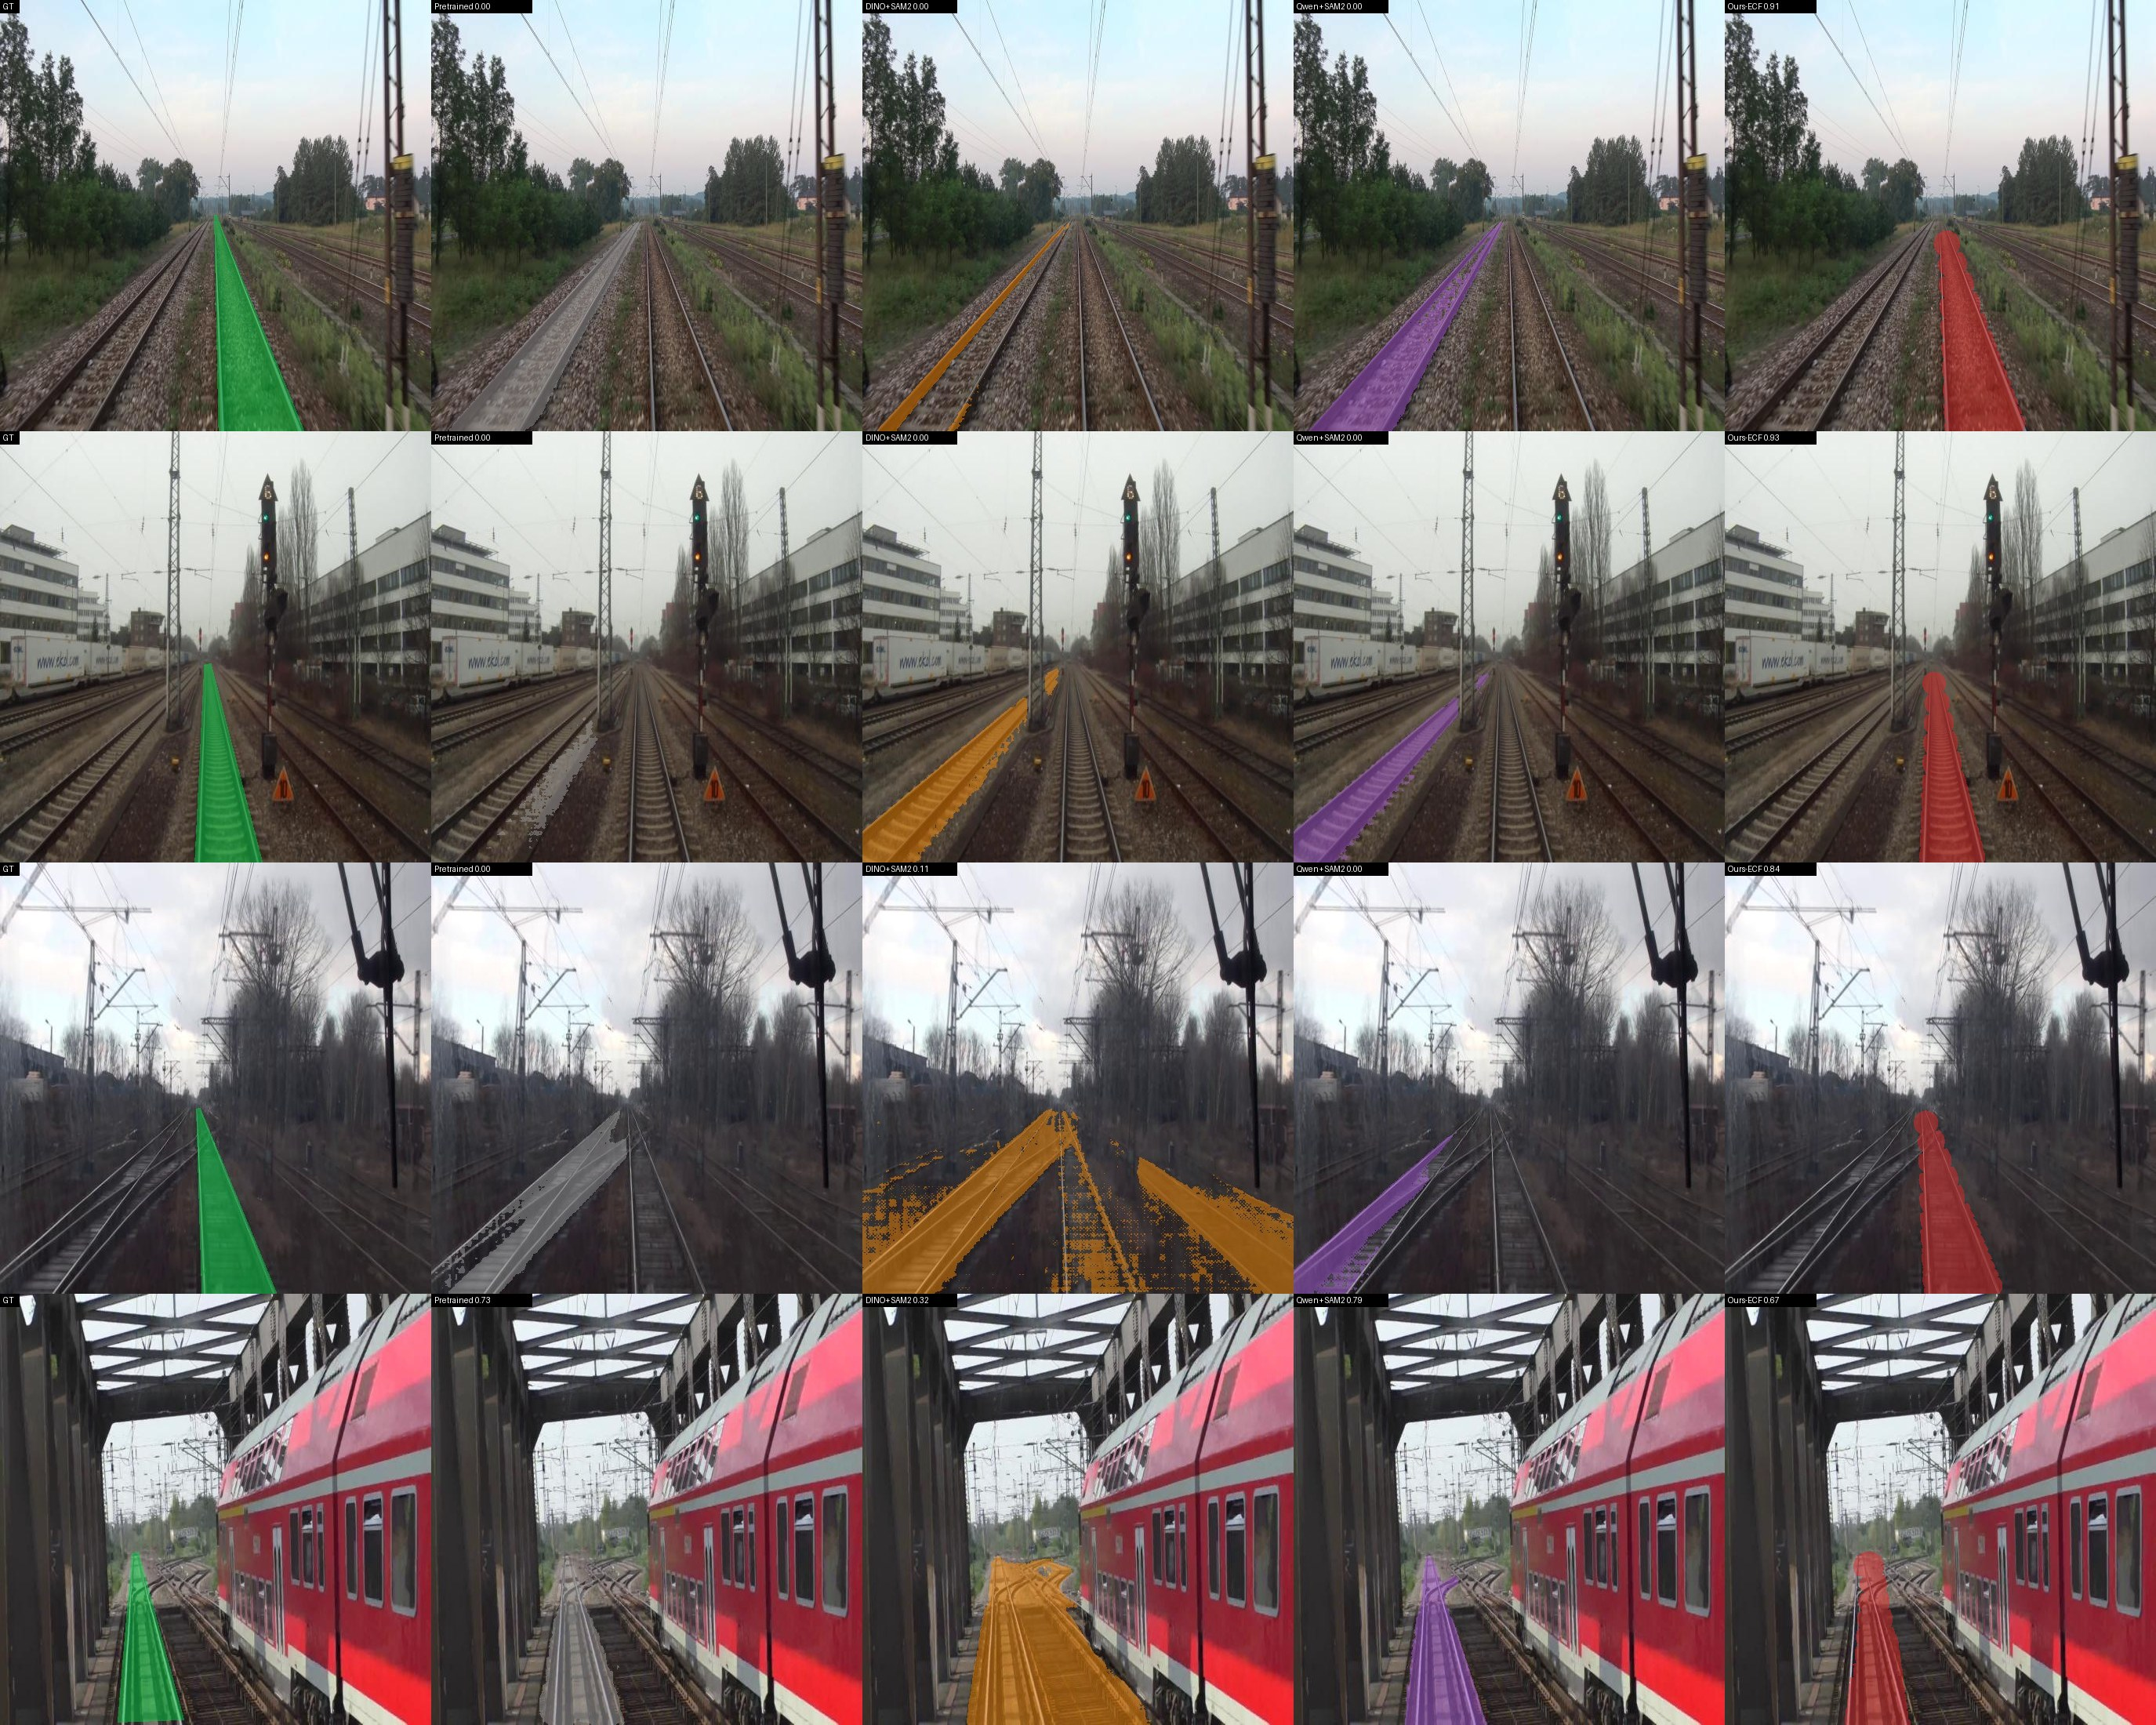
\includegraphics[width=\textwidth]{figures/fig1_qual.jpg}%
}{\fbox{\parbox{0.95\textwidth}{\centering\vspace{16mm}Qualitative panel pending.\vspace{16mm}}}}
\caption{Qualitative comparison on FIRC test (fp32). Columns: GT, pretrained Sa2VA, GroundingDINO+SAM2, Qwen2.5-VL-7B+SAM2, and our ECF-native rasterization. Panel labels give the per-image IoU of that column (two decimals). Panel labels come from the same evaluation runs as Table~\ref{tab:main}, so the figure and the table cannot disagree. In rows 1--3 both detector pipelines return no usable mask (0.00) or a small spurious one (0.11) on the ordinal caption, while ECF recovers a vanishing-point-aligned rail mask. Row 4 shows why a table of means alone is not enough: Qwen2.5-VL (0.79) and pretrained Sa2VA (0.73) do produce high-IoU masks, but on the \emph{wrong} rail: the target-selection failure that a mean score hides, and the failure mode ECF is built to avoid.}
\label{fig:qual}
\end{figure*}


\subsection{The rasterization loop is not optional}
\label{sec:ablate}

Table~\ref{tab:ablate} isolates the two falsifiers of the carrier claim; they are the A1/A2 panels of Figure~\ref{fig:framework}.
A1 doubles as the \emph{matched-training control} for Table~\ref{tab:main}: it reuses the trained LoRA and ParamHead of the main row and changes only the mask carrier, so any gap it shows is attributable to the carrier rather than to the mere presence of fine-tuning, and Table~\ref{tab:diag} shows the same falsifiers plus the width-profile limitation, one row per mechanism.

\paragraph{A1: same weights, SAM2 decode.}
We keep the ECF LoRA and ParamHead and instead route the \Seg{} embedding through SAM2, as a standard Sa2VA mask.
gIoU falls to 2.43, \PrAt{0.5} to 0.96 and \PrAt{0.7} to 0.0; TinyMaskRate (predicted mask under $0.1\%$ of the image area) is 30.29\%.
The embeddings that produce a corridor under $\cR$ are \emph{not} valid SAM2 prompts: this is the empirical counterpart of DeSa2VA's observation that extra signal into an entangled SAM2 pathway is not free, since here the extra signal is geometric and SAM2, as trained, does not read it.
It is also what rules out the trivial reading of Table~\ref{tab:main}, namely that ``fine-tuning simply helps'', because fine-tuning the same backbone and head with our recipe and then decoding with the original SAM2 carrier does not recover the gain.

\paragraph{A2: train without raster mask loss.}
An architecture-identical ECF model trained with $\lambda_{\mathrm{mask}}{=}0$ (parameter loss only; same orig$\cup$hflip schedule) reaches gIoU 69.31, \PrAt{0.5} 94.71, and \PrAt{0.7} \textbf{54.81}.
The head still emits a corridor-shaped region that often crosses IoU 0.5, but its high-IoU rate falls sharply: \PrAt{0.7} drops from 87.98 to 54.81, and pixel supervision through $\cR$ is the term that delivers \PrAt{0.7}---33.2 points above the no-mask-loss arm; $\phih^{gt}$ alone is not a substitute.

\begin{table}[t]
\centering
\small
\setlength{\tabcolsep}{3pt}
\caption{Carrier ablations on FIRC test ($n{=}208$, fp32). Row 1 is the main trained model. A1 reuses those trained LoRA/ParamHead weights with the SAM2 decoder and is the matched-training control for Table~\ref{tab:main}. A2 is an architecture-identical retrain with $\lambda_{\mathrm{mask}}{=}0$ on the same orig$\cup$hflip schedule.}
\label{tab:ablate}
\begin{tabularx}{\columnwidth}{@{}Ycccc@{}}
\toprule
Setting & \gIou & \PrAt{0.5} & \PrAt{0.7} & SegRate \\
\midrule
\textbf{ECF-native $\cR$} & \textbf{80.67} & \textbf{97.6} & \textbf{87.98} & 100.0 \\
A1: same weights $\to$ SAM2 & 2.43 & 0.96 & 0.0 & 100.0 \\
A2: $\lambda_{\mathrm{mask}}{=}0$ retrain & 69.31 & 94.71 & 54.81 & 100.0 \\
\bottomrule
\end{tabularx}
\end{table}

On the main run, 203/208 frames reach IoU ${\ge}0.5$ and 183/208 reach IoU ${\ge}0.7$; SegRate is 100\%, so every frame receives a mask.
Residual errors are geometric (thin far-field, boundary jitter), not detector-style empty masks, consistent with Figure~\ref{fig:qual}, and Figure~\ref{fig:ph_ecf_teaser} shows the same carrier over four ego-view rail settings.
On the same frames, the off-the-shelf reference systems fail in two different ways.
On the ordinal captions their masks are absent or negligible (Figure~\ref{fig:qual}, rows 1--3: 0.00 for both pipelines, and 0.11 for GroundingDINO+SAM2 in one case), so the mean in Table~\ref{tab:main} understates how rarely they solve the task at all; on the harder frame of row 4 they do return confident masks (Qwen2.5-VL at 0.79 and pretrained Sa2VA at 0.73) but on a different rail than the one the caption names.
A mean over gIoU cannot always separate ``found the referred rail'' from ``found a rail'': in row 4, the masks are confident yet land on the wrong rail, a target-selection failure under language rather than a mask-quality one.

Figure~\ref{fig:display} turns to the complementary diagnostic question of whether the $20$-D carrier can represent the referred corridor at all, across the shapes that occur in this split.
Each column shows one test frame with its ground-truth rail and the field reconstructed back to a mask, and each chip reports the \emph{reconstruction} IoU of that label-derived field against the ground-truth mask; it is a property of the carrier, not a model accuracy.
Corridors span the multi-rail ordinal case, the widest near-field in the split ($0.56$), and an occluded platform edge ($0.86$); over the $208$ test frames the reconstruction median is $0.891$ (supplementary material, Section~D).
Where the carrier is weakest, namely thin far-field and boundary jitter, is also where our residual error concentrates, which is the geometric failure mode claimed in Section~\ref{sec:ablate}.

\begin{figure*}[t]
\centering
\IfFileExists{figures/fig5_rail_qual.png}{%
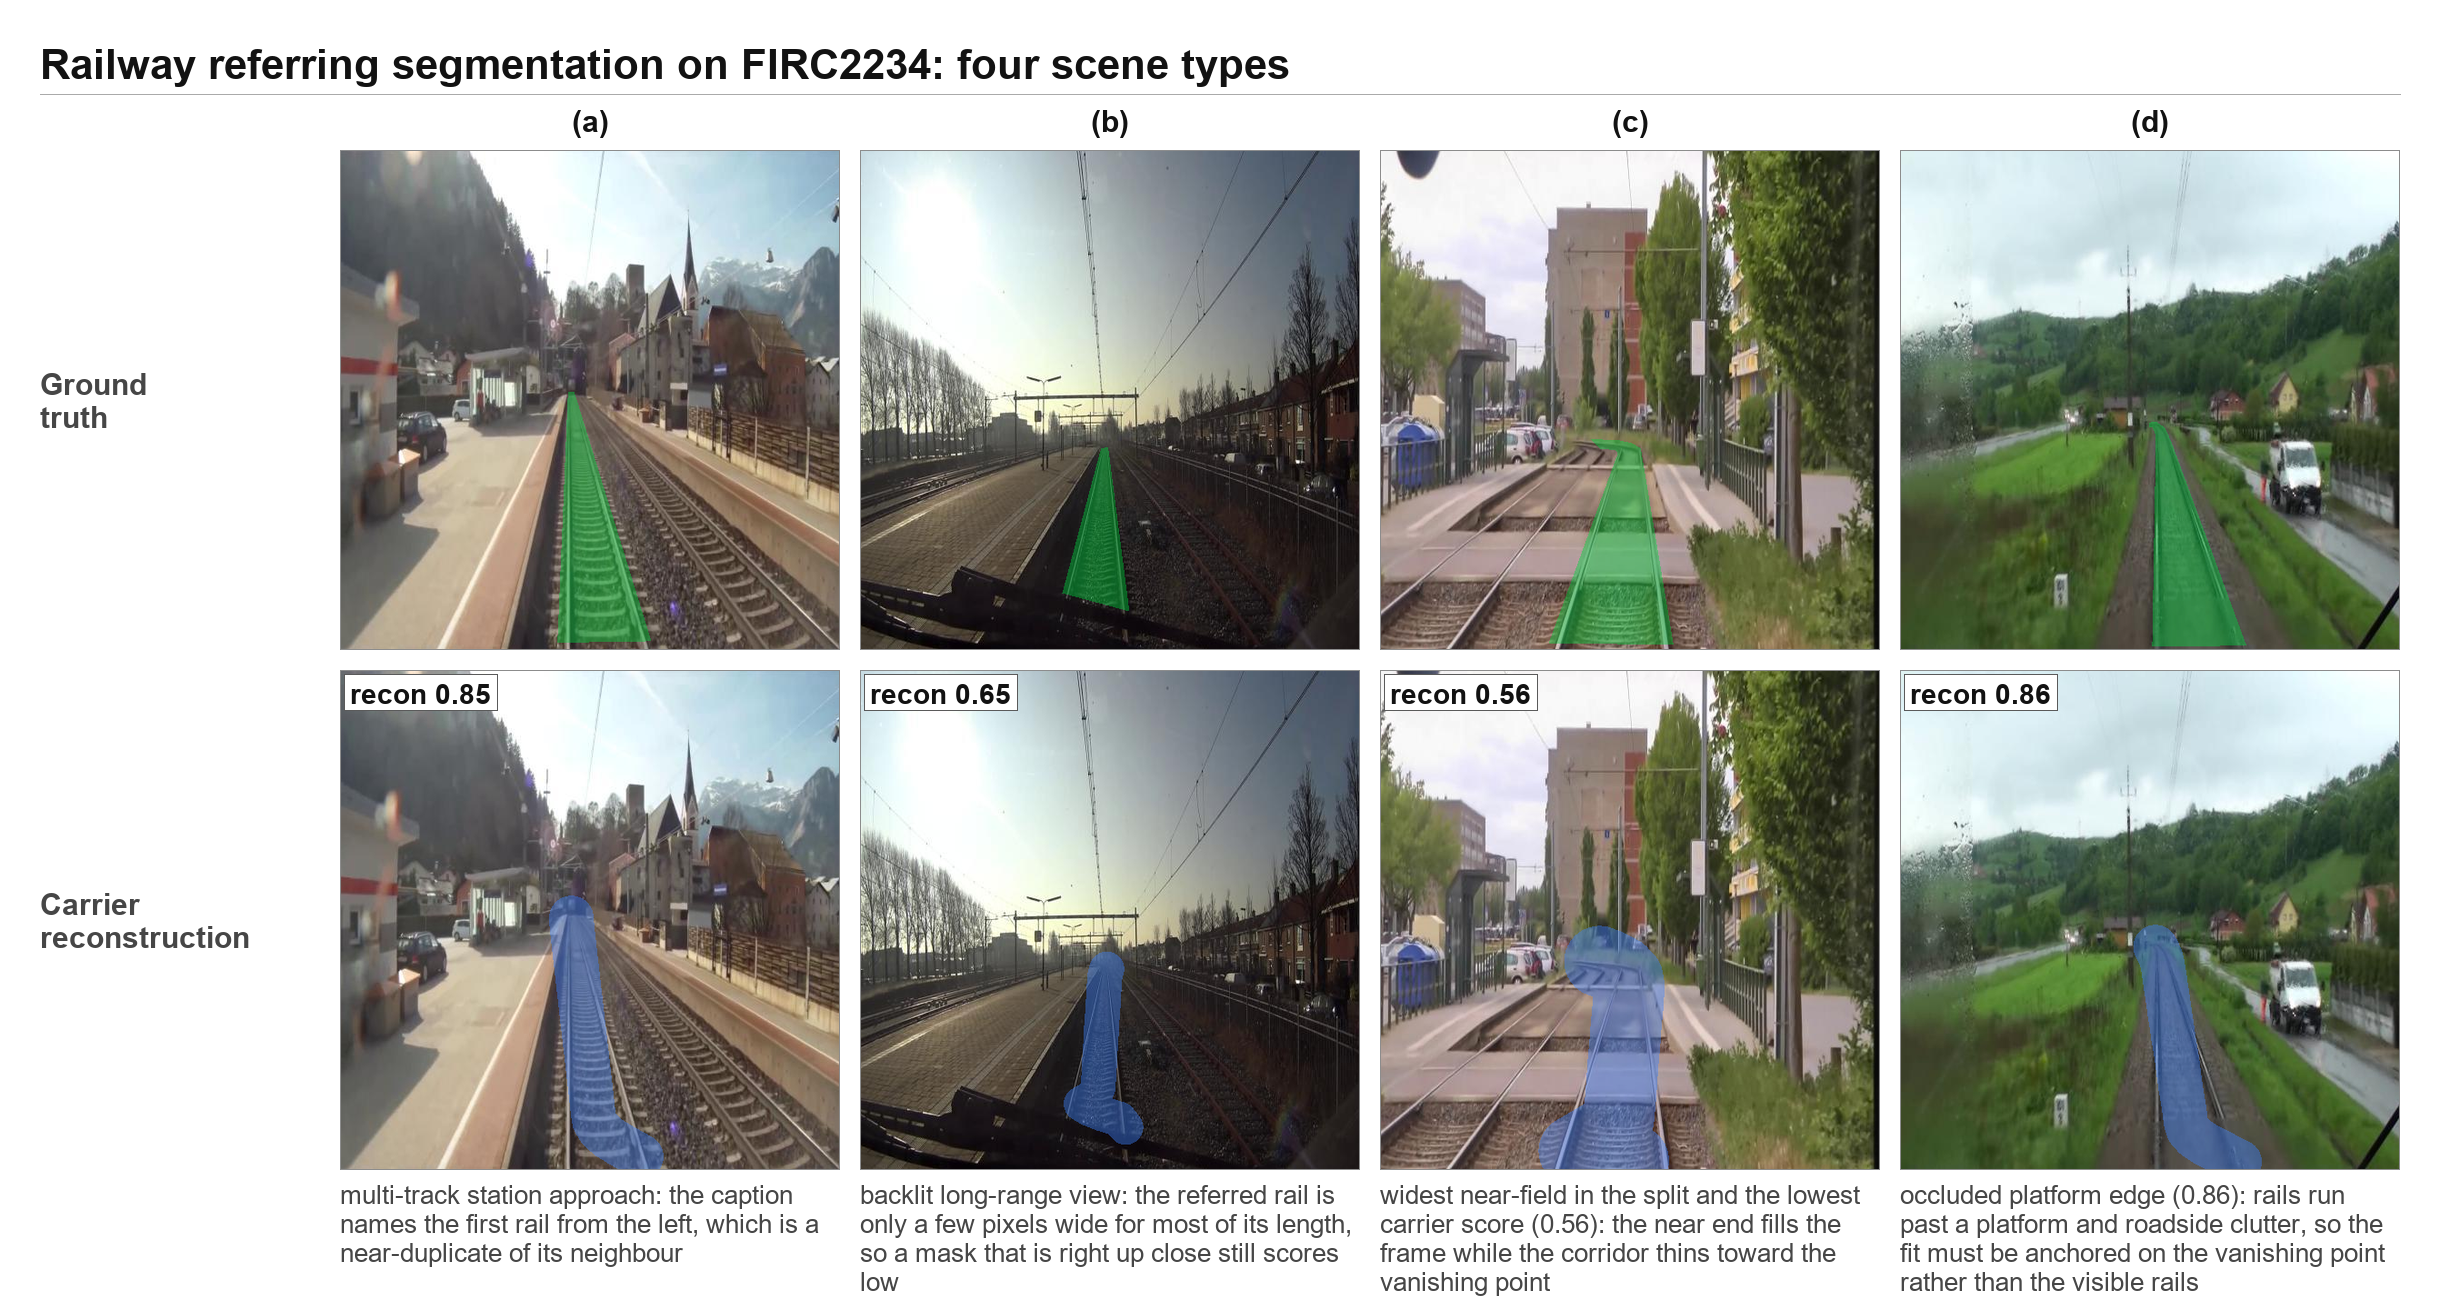
\includegraphics[width=\textwidth]{figures/fig5_rail_qual.png}%
}{%
\fbox{\parbox{0.95\textwidth}{\centering\vspace{14mm}Railway qualitative panel omitted in this build.\vspace{14mm}}}%
}%
\caption{What the carrier has to cover (FIRC2234 test, fp32 protocol).
Rows: the ground-truth referred rail and the reconstruction of the label-derived corridor carrier, both drawn as a translucent tint over the rails so the \emph{which rail} question stays visible.
Columns: one scene per challenge, labeled (a)--(d) as in the railway-segmentation literature, chosen to span the split.
(a)~a multi-track station approach, where the caption's ``first from left'' must be separated from near-duplicate neighbors ($0.85$);
(b)~a backlit long-range view, where the referred rail spans only a few pixels over most of its length ($0.65$);
(c)~the widest near-field frame in the split, where the near end fills the frame while the corridor thins toward the vanishing point ($0.56$);
(d)~an occluded platform edge, where the fit must be anchored on the vanishing point rather than the visible rails ($0.86$).
Chips give the per-frame \emph{recon IoU}, the reconstruction of the label-derived field against the ground-truth mask (median $0.891$ over $n{=}208$).
It measures the \emph{label} under the non-learned label-QA renderer of the supplementary material (Section~D), not the differentiable $\cR$ used in training, and is not comparable to Table~\ref{tab:main}.
Tiles are rendered from the dataset annotations and the corridor-label records; no model output enters this figure.
The panel is shared with the companion submission by the same authors and has not appeared elsewhere.}
\label{fig:display}
\end{figure*}

% ---------------------------------------------------------------------------
% [TABLE] carrier diagnostics -- converted from the former figure ecf_analysis_redraw.png
% ---------------------------------------------------------------------------
\begin{table}[t]
\centering
\small
\setlength{\tabcolsep}{3pt}
\caption{Three diagnostics that isolate what the loop removes (FIRC test, fp32, $n{=}208$). Rows (a)/(b) are the two falsifiers of Table~\ref{tab:ablate}; row (c) records the width-profile limitation: the rasterizer consumes only the per-side mean of the stored width samples, so a width profile along the corridor is deliberately not represented.}
\label{tab:diag}
\begin{tabularx}{\columnwidth}{@{}YYY@{}}
\toprule
Diagnostic & Setting & Result \\
\midrule
(a) raster carrier, not SAM2 decode & same trained $h$, SAM2 decode & $80.67 \to 2.43$ \gIou \\
(b) mask loss off & $\lambda_{\mathrm{mask}}{=}0$ retrain & $69.31$ \gIou, $\PrAt{0.7}{=}54.81$ \\
(c) width profile & per-side mean only & envelope not represented \\
\bottomrule
\end{tabularx}
\end{table}

Table~\ref{tab:diag} isolates, one row at a time, the elements that the loop removes.


\subsection{Eval-only transfer and harder captions}
\label{sec:transfer}

The FIRC checkpoint is frozen, and Table~\ref{tab:transfer} reports two additional single-rail fill-band protocols, each with its own off-the-shelf reference set (never copied from Table~\ref{tab:main}).
RailSem19-EgoPair keeps frames with exactly one polyline pair ($n{=}300$ test) and RailBench 1L1R keeps frames with exactly one left and one right rail polyline ($n{=}260$); neither set is used for training, and ECF keeps the best gIoU on each protocol (66.93 vs.\ 41.90 on EgoPair; 54.21 vs.\ 46.35 on RailBench).

\begin{table*}[t]
\centering
\small
\setlength{\tabcolsep}{4pt}
\caption{Eval-only transfer. Not mixed into Table~\ref{tab:main}. Caption template matches FIRC. Reference rows are off-the-shelf systems; ECF rows reuse the frozen FIRC checkpoint with no further training (EgoPair $n{=}300$; RailBench 1L1R $n{=}260$).}
\label{tab:transfer}
\begin{tabularx}{\textwidth}{@{}Ycccc@{}}
\toprule
Protocol / method & \gIou & \PrAt{0.5} & \PrAt{0.7} & SegRate \\
\midrule
EgoPair, pretrained Sa2VA & 12.48 & 8.67 & 5.67 & 100.0 \\
EgoPair, GroundingDINO+SAM2 & 41.90 & 41.33 & 33.67 & 99.3 \\
EgoPair, Qwen2.5-VL-7B+SAM2 & 38.93 & 42.67 & 31.33 & 100.0 \\
\textbf{EgoPair, ECF (FIRC ckpt)} & \textbf{66.93} & \textbf{94.00} & \textbf{45.67} & 100.0 \\
\midrule
RailBench 1L1R, pretrained Sa2VA & 16.46 & 16.92 & 9.23 & 100.0 \\
RailBench 1L1R, GroundingDINO+SAM2 & 46.35 & 49.62 & 38.08 & 99.2 \\
RailBench 1L1R, Qwen2.5-VL-7B+SAM2 & 7.07 & 7.31 & 6.15 & 100.0 \\
\textbf{RailBench 1L1R, ECF (FIRC ckpt)} & \textbf{54.21} & \textbf{70.38} & \textbf{31.92} & 100.0 \\
\bottomrule
\end{tabularx}
\end{table*}

\paragraph{On linguistic control.}
A natural concern about a single-rail set is that the model may ignore the caption and segment the only rail present.
FIRC2234 cannot settle this: every test frame carries the same caption string, and a caption that names a non-existent neighboring branch cannot be scored as an instance switch (Table~\ref{tab:data}).
What we can show is insensitivity to a same-target paraphrase: with harder rephrasings of the \emph{same} target (same masks), ECF stays at 80.97 gIoU (Table~\ref{tab:hardref}), within 0.3 points of the 80.67 obtained with the original caption.
A caption-swap probe, which feeds one frame the caption of a \emph{different} target and checks that the predicted mask moves, requires multi-rail frames with distinct per-rail captions, which FIRC2234 does not contain; we therefore flag it as the most important missing experiment for a linguistic-control claim (Section~\ref{sec:conclusion}) rather than over-read the paraphrase table.

\begin{table}[t]
\centering
\small
\setlength{\tabcolsep}{3pt}
\caption{Same FIRC test masks, harder same-target paraphrases ($n{=}208$, fp32). This is a robustness probe, not a linguistic-sensitivity test; see the text.}
\label{tab:hardref}
\begin{tabularx}{\columnwidth}{@{}Ycccc@{}}
\toprule
Caption / method & \gIou & \PrAt{0.5} & \PrAt{0.7} & SegRate \\
\midrule
Hard-ref, pretrained Sa2VA & 4.80 & 5.29 & 2.88 & 100.0 \\
\textbf{Hard-ref, ECF} & \textbf{80.97} & \textbf{97.60} & \textbf{86.54} & 100.0 \\
\bottomrule
\end{tabularx}
\end{table}
